% LTeX: language=de-DE
\section{Lexikalische \& Syntaktische Analyse}

\begin{frame}{Etappen der Übersetzung: Semantische Analyse}
	\pdfpcnote{
		@Silas \\
		\\
		- In jedem Fall sind die ersten Schritte die lexikalische und syntaktische Analyse \\
		- bei rush zu einem Schritt zusammengefasst \\
	}

	\begin{figure}[h]
		\begin{adjustbox}{max totalsize={\textwidth}{!},center}
			\begin{tikzpicture}[node distance=3mm and 1cm, inner sep=3mm]
				\node (syntactic_analysis_text) [inner sep=0] {Syntaxanalyse};
				\node (lexical_analysis) [rec, below=of syntactic_analysis_text] {Lexikalische Analyse};
				\begin{scope}[on background layer]
					\node (syntactic_analysis) [rec, fill=mLightBrown!35, fit={(syntactic_analysis_text) (lexical_analysis)}] {};
				\end{scope}
				\node (semantic_analysis) [rec, right=of syntactic_analysis] {Semantische Analyse};
				\draw [arrow] (syntactic_analysis) -- (semantic_analysis);
				\node (codegen) [rec, right=of semantic_analysis] {Code-Erzeugung};
				\draw [arrow] (semantic_analysis) -- (codegen);
			\end{tikzpicture}
		\end{adjustbox}
	\end{figure}
\end{frame}

\begin{frame}{Lexikalische \& Syntaktische Analyse}
	\pdfpcnote{
		@Silas \\
		\\
		- Programmtext wird in sogenannte _Tokens_ gruppiert (lex. analyse) \\
		- darauf basierend: **die** Syntax des Programms wird analysiert \\
		- dabei: ein abstrakter Syntaxbaum wird erstellt \\
		- **die** Syntax ist formal in Form einer Grammatik definiert \\
		- Beispiel fuer solch eine Grammatik \\
		- die rush Grammatik ist deutlich laenger \\
	}

	\begin{itemize}
		\item Gruppieren des Programmtextes in Tokens
		\item Analyse der Syntax des Programms
		\item Erzeugung eines abstrakten Syntaxbaums
		\item Festlegen der formalen Regeln in Form einer Grammatik
	\end{itemize}

	\raggedleft
	\begin{minipage}{0.955\textwidth}
		\Lirsting[float=H, fancyvrb={frame=none, fontsize=\small}]{listings/grammar.ebnf}
	\end{minipage}
\end{frame}

\begin{frame}{Abstrakter Syntaxbaum}
	\pdfpcnote{
		@Silas \\
		\\
		- sichtbar: zwei verschiedene Syntaxbaeume \\
		- beide fuer den Ausdruck `1+2**3` \\
		- unterschiedlich weil: Verwendung verschiedener Algorithmen \\
		- rechts geringere Tiefe -> wuenschenswert \\
	}

	\begin{figure}[h]
		\begin{minipage}{.45\textwidth}
			\raggedleft
			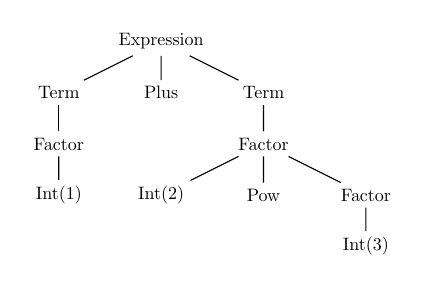
\begin{tikzpicture}[level distance=1cm, sibling distance=2cm, scale=.65, transform shape]
				\node {Expression}
				child {node {Term}
						child {node {Factor}
								child {node {\Verb{Int(1)}}}}}
				child {node {\Verb{Plus}}}
				child {node {Term}
						child {node {Factor}
								child {node {\Verb{Int(2)}}}
								child {node {\Verb{Pow}}}
								child {node {Factor}
										child {node {\Verb{Int(3)}}}}}};
			\end{tikzpicture}
		\end{minipage}
		\hfill
		\begin{minipage}{.45\textwidth}
			\raggedright
			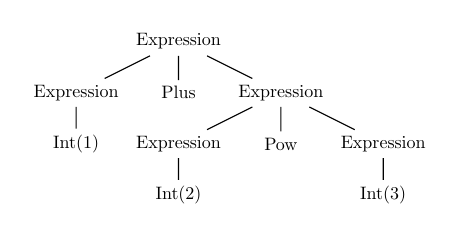
\begin{tikzpicture}[level distance=1cm, sibling distance=2cm, scale=.65, transform shape]
				\node {Expression}
				child {node {Expression}
						child {node {\Verb{Int(1)}}}}
				child {node {\Verb{Plus}}}
				child {node {Expression}
						child {node {Expression}
								child {node {\Verb{Int(2)}}}}
						child {node {\Verb{Pow}}}
						child {node {Expression}
								child {node {\Verb{Int(3)}}}}};
			\end{tikzpicture}
		\end{minipage}

		\centering
		Zwei verschiedene Syntaxbäume für \enquote{\LirstInline{rush}{1+2**3}}
	\end{figure}
\end{frame}
